\documentclass{article}
\usepackage[utf8]{inputenc}
\usepackage{authblk}
\usepackage{amsmath}
\usepackage{amssymb}
\usepackage{graphicx}
\usepackage{physics}
\usepackage{float}
\usepackage{bm}
\usepackage{caption}
\usepackage{subcaption}
\usepackage{dsfont}
\usepackage[parfill]{parskip}
\usepackage{blkarray}
\usepackage[dvipsnames]{xcolor}
\usepackage[most]{tcolorbox}

\newcommand{\Id}{\mathds{1}}
\newcommand\sj[1]{ {\color{orange} #1} } 


\newcommand{\matindex}[1]{\mbox{\scriptsize#1}}% Matrix index
\usepackage{geometry}
 \geometry{
 a4paper,
 left=25mm,
 right = 25 mm,
 top = 15mm,
 }


\title{QPC Project Status to 08.2025: Schmidt Decomposition and more Perturbation}
\author{Santiago Salazar Jaramillo}
\date{}


\begin{document}
\maketitle

In the previous update, we focused on the perturbative expansion for the composite QPC-qubit eigenstates 
\begin{align}
    \ket{\phi_\nu (k)} = \ket{\phi_\nu^{(0)} (k)} + \Omega \ket{\phi_\nu^{(1)} (k) },
\end{align}
where $\ket{\phi_\nu^{(0)} (k)} = \ket{k}\otimes\ket{\nu}$ as given in Eqs.\eqref{eq:QPC_eigenstates}  and \eqref{eq:qubit_eigensates}. The first order correction Eq.\eqref{eq:psi_1} was found to have a \textit{band-mixing term},
 describing the QPC-qubit scattering interactions. Most important are the states at which this term becomes degenerate (whenever $\epsilon_\nu = 2J(\cos k -\cos p)$), since these should yield the largest contributions to entanglement. The following text focuses on testing this hypothesis. All the results shown below use $J=1$ as the QPC hopping.


 \begin{tcolorbox}[title=QPC eigenstates, colback=white, colframe=black]
\begin{align}\label{eq:QPC_eigenstates}
    \bra{j}\ket{k} = \sqrt{\frac{2}{N+1}} \sin(j k) ,\quad & E(k) = -2J\cos(k), \quad k = \frac{j\pi}{N+1},\quad j= 1, 2,...N
\end{align}
Here $\ket{j}$ is the position basis and $\ket{k}$ is the momentum basis.
\end{tcolorbox}

\begin{tcolorbox}[title=Qubit eigenstates, colback=white, colframe=black]
\begin{align}\label{eq:qubit_eigensates}
   & \ket{+} = \frac{1}{\sqrt{2}}\left( \ket{0} + e^{i\phi} \ket{1}\right), \quad \epsilon_+ = t \nonumber \\
   & \ket{-} = \frac{1}{\sqrt{2}}\left( \ket{0} - e^{i\phi} \ket{1}\right), \quad \epsilon_- = -t, 
\end{align}
where $+$ labels the symmetric state and $-$ the antisymmetric one and $t$ is the Rabi frequency.
\end{tcolorbox}

\section{The fast qubit}

 First, let us focus on the case where $t>J$, i.e. the \textit{fast qubit regime}. Here, there are no degeneracies as $|\epsilon_\nu|$ is always bigger than $|J \cos(k)|$, so entanglement is expected to vanish the larger $t$ becomes. 

\begin{align}\label{eq:psi_1}
    \ket{\phi_\nu^{(1)} (k)} = & \frac{1}{(N+1)}\sum_{p\neq k} \ket{p}\otimes \left \{ \frac{ \xi(k,p)}{ -2J( \cos k - \cos p ) } \ket{\nu} + \overbrace{\frac{ \xi(k,p)}{ 2\epsilon_\nu -2J( \cos k - \cos p )} \ket{\mu}}^{\text{Band mixing term}} \right \} \nonumber \\ 
    & + \frac{1}{(N+1)} \frac{\xi(k,k)}{2\epsilon_\nu} \ket{k}\otimes\ket{\mu},
\end{align}

We calculated data points up until $t=3$ using our qutip, exact diagonalization algorithm and extended the $t$ vs $k_0$ (where $k_0$ is the wavepacket central momentum) phase diagram we had. The heatmap shown in Figure \ref{fig:S_phase_diagram} clearly shows that the entropy becomes smaller as $t>J$. In fact at around $t=2.5$ the entanglement effectively vanishes as it also does when $t\rightarrow 0$. 

\begin{figure}[h]
    \centering
        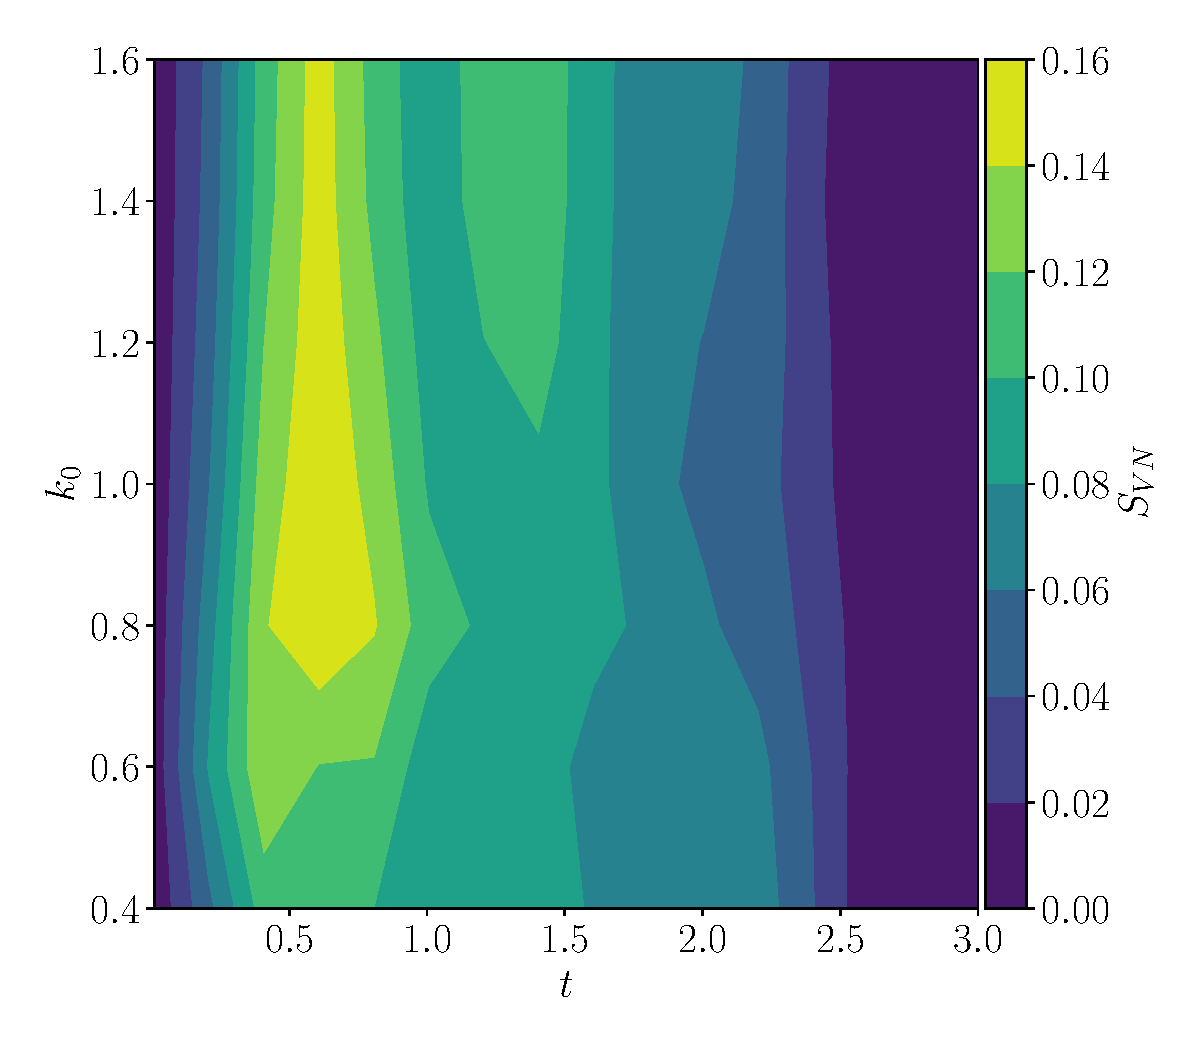
\includegraphics[width=0.46\textwidth]{figures/report_08_2025/entropy_phase_diagram_L_=21_bw=2.0_Jp=1.0_om=0.3.pdf}
    \caption{Phase diagram of the Von Neumann entropy $S_{\rm{VN}}$, for a QPC of size $L=21$ $J=1$ and coupling $\Omega=0.3$.}
    \label{fig:S_phase_diagram}
\end{figure}

We believe this is due to the qubit oscillations being so fast, that the comparatively slow QPC dynamics effectively "feels" a constant occupation on the interacting site. This situation is equivalent to scattering of a constant potential ($t=0$) which generates no entanglement.

\section{The slow qubit and Schmidt decomposition}

The case where $t<J$ is more complicated than the fast qubit regime. As pointed out in the previous report, Eq.\eqref{eq:psi_1} becomes degenerate whenever $ \cos p = \pm t/J + \cos k$, from which conditions \eqref{eq:scattering_condition} and \eqref{eq:band_gap_condition} are deduced. Combining both of them determines which states are capable of being degenerate and contribute significantly to the entropy. 

\begin{tcolorbox}[title=Scatering Condition, colback=white, colframe=black]
Only $k$-momenta that fulfill
\begin{align}\label{eq:scattering_condition}
    & \text{For the symmetric band ($\nu = +$): } -1 \leq \frac{t}{J} + \cos{k} \leq 1 \\
    & \text{For the anti-symmetric band ($\nu = -$): } -1 \leq -\frac{t}{J} + \cos{k} \leq 1
\end{align}
can contribute to the degeneracy, otherwise $\cos p= \pm t/J + \cos k$ has no solution.
\end{tcolorbox}

\begin{tcolorbox}[title=Band-Gap condition, colback=white, colframe=black]
    The perturbative expansion \eqref{eq:psi_1} is well-behaved only when $2\epsilon_\nu \neq \Delta E(k)$. This is always true, when $t/J>1$ and near the middle of the band when
\begin{align}\label{eq:band_gap_condition}
    \frac{t}{J}<\frac{\pi}{N+1}, \quad \text{ For $k\approx\pi/2$ }.
\end{align}
\end{tcolorbox}

To further test these conditions, we calculate the entanglement entropy of each eigenstate by using the Schmidt decomposition. First, we write down the exact eigenstate of the full interacting QPC-qubit system as
\begin{align}\label{eq:schmidt_eigenstates}
    \ket{\phi_\nu (k)} = \sum_{j,q} \phi_{j,q} (\nu, k) \ket{\vec{j}}_{\rm{QPC}}\otimes\ket{q}_{\rm{qubit}} = \sum_{j,q} \phi_{j,q} (\nu, k) \ket{\vec{j},q},
\end{align}
where $j$, $q$ \textit{always} refer to the QPC/qubit site and $\phi_{j,q} (\nu, k) = \bra{\vec{j},q} \ket{\phi_\nu (k)}$. The vector notation over the QPC lattice index $j$ is understood as labelling the site where the particle is located
\begin{align}
    \ket{\vec{j}} = \ket{00 \hdots \overbrace{1}^{j\text{-th site}} \hdots 0}
\end{align}
running from $1$ to $L$. On the other hand $q=0,1$ just labels the states of the qubit. The advantage of writing the eigenstate in this form is that, it already is a Matrix Product State (MPS) with a bipartition separating the QPC chain and the qubit. Hence, the Schmidt representation is found by applying an SVM to the ($L\times 2$) tensor whose elements are $\phi_{j,q}(\nu,k)$. In matrix form one can write
\begin{align}
    \Phi(\nu, k) = 
    \begin{pmatrix}
        \phi_{1,0}(\nu,k) & \phi_{1,1}(\nu,k) \\
        \phi_{1,0}(\nu,k) & \phi_{1,1}(\nu,k) \\
        \vdots & \vdots                        \\
        \phi_{L,0}(\nu,k) & \phi_{L,1}(\nu,k)
    \end{pmatrix}
\end{align}
by placing the QPC indices as the rows and the qubit ones as the columns. Then, applying the SVM decomposition $\Phi(\nu, k) = U S V^{\dagger}$, where $S$ is the diagonal $L\times 2$ matrix with entries $\lambda_{l}(\nu,k)$ known as the Schmidt coefficients. Therefore, the state is rewritten in its Schmidt decomposition as 
\begin{align}
    \ket{\phi_\nu (k)} = \sum_{l=1}^{2} \sqrt{\lambda_l(\nu,k)} \left( \sum_{j=1}^{L} U_{j,l} \ket{\vec{j}} \right)\otimes \left( \sum_{q=0}^{1} V_{l,q}^{\dagger} \ket{q} \right).
\end{align}
Therefore, the entanglement entropy contributed by the state $\ket{\phi_\nu (k)}$ is
\begin{align}
    S_{\rm{VN}}(\nu,k) = - \sum_{l=1}^{2} \lambda_l(\nu,k)  \log(\lambda_l(\nu,k)). 
\end{align}
Given that, the exact analytic form of the QPC-qubit eigenstates is not known, we use numpy's numerical exact diagonalization routine to calculate $\phi_{j,q}(\eta,k)$ and calculate the entropy. The results are shown in figure \ref{fig:energy_bands} on top of the energies $E_\nu(k)$ from the exact diagonalization. In this figure, everything is color coded: red refers to the antisymmetric band while blue to the symmetric one. Furthermore, the size of the QPC chain $L=60$ means that the RHS of Eq.\eqref{eq:band_gap_condition} is $\approx 0.52$ and the two values of $t$ where chosen such that one case fulfills it and the other does not. 

\begin{figure}[h]
    \centering
    \begin{subfigure}[b]{0.43\textwidth}
        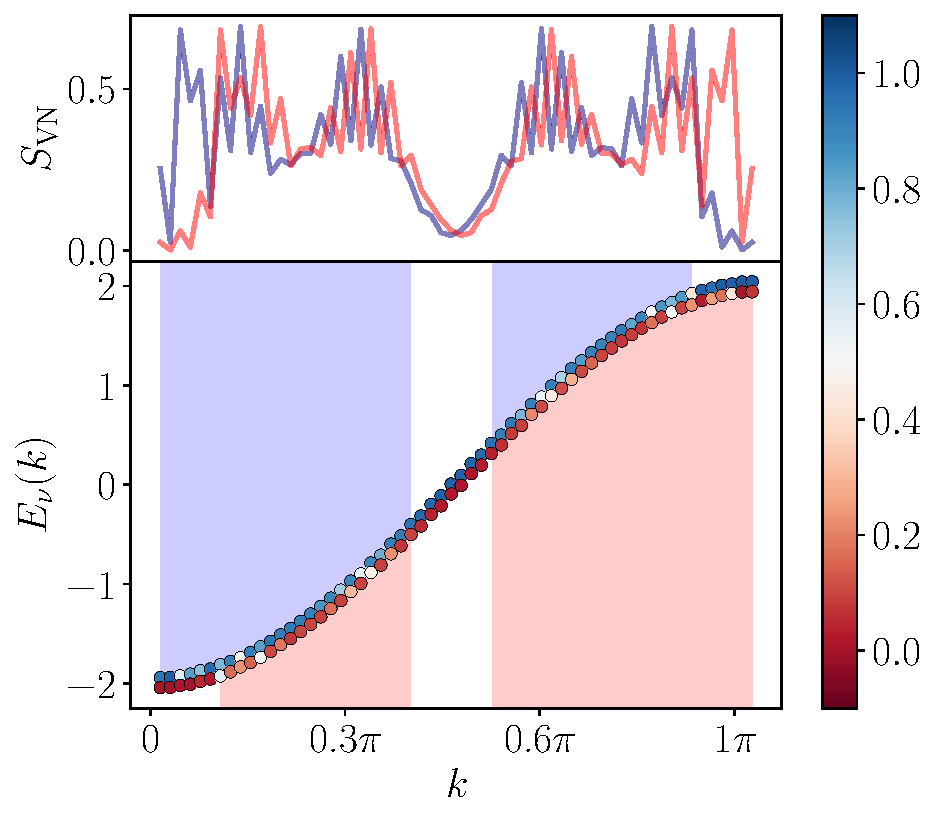
\includegraphics[width=\textwidth]{figures/report_08_2025/exact_energies_Lqpc=60_Omega=0.4_t=0.05.pdf}
        \caption{}
    \end{subfigure}
    \hspace{0.001\textwidth}
    \begin{subfigure}[b]{0.43\textwidth}
        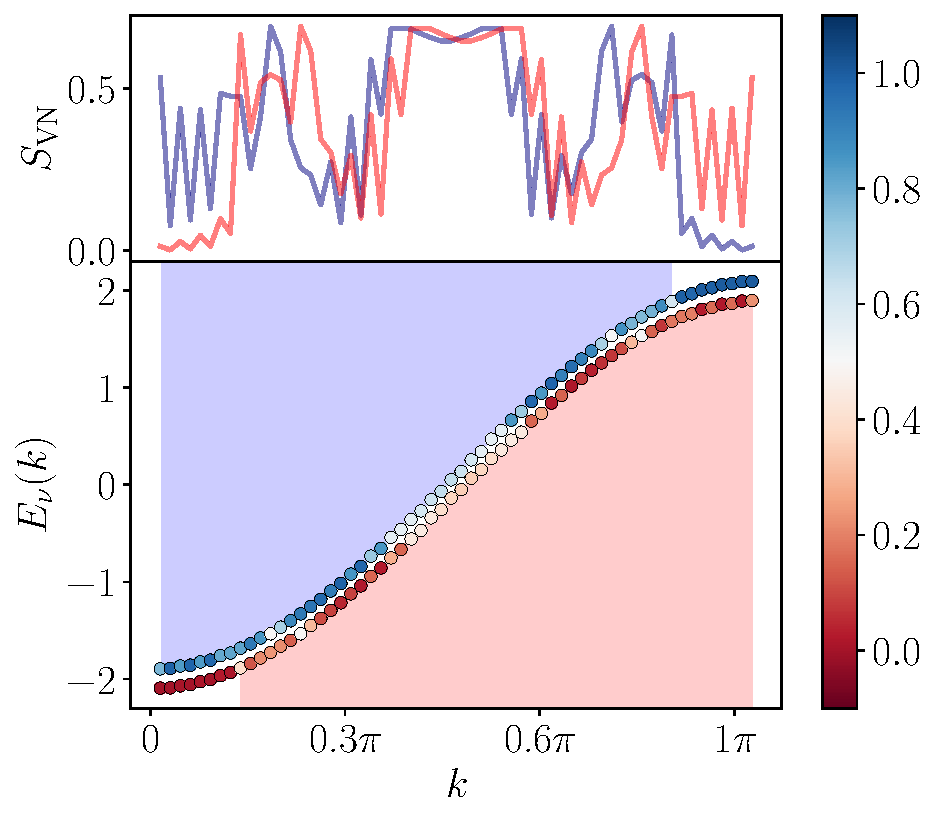
\includegraphics[width=\textwidth]{figures/report_08_2025/exact_energies_Lqpc=60_Omega=0.4_t=0.1.pdf}
        \caption{ }
    \end{subfigure}
    \caption{Exact band structure and entropy contributions of the coupled systems for a QPC of size $L=60$ and $\Omega=0.4$, where (a) depicts the case with Rabi frequency $t=0.05$ and (b) with $t=0.1$. The upper plot shows the entropy that each eigenstate $\ket{\phi_\nu (k)}$ contributes, with the blue line corresponding to the symmetric band and the red line to the antisymmetric one. Both are normalized by the entropy of a singlet $S_{\rm{max}}=\log{2}$. The lower plot shows the eigenenergies sorted into bands, where the color corresponds to the projection of the eigenstate onto the symmetric (blue) and antisymmetric (red) states. The (also color-coded) shaded areas indicate the regions where the perturbative expansion \eqref{eq:psi_1} is degenerate, according to conditions Eq.\eqref{eq:scattering_condition} and Eq.\eqref{eq:band_gap_condition}.}
    \label{fig:energy_bands}
\end{figure}

Importantly, the predictions from perturbation theory as to where the expansion is degenerate (shaded regions), correspond both to higher entropy contributions and to stronger band mixing (Lighter colors in the energies). This is clearly seen in the case where $t=0.05$, where the expansion is less degenerate in the middle of the chain. Regarding the edges, it is also clear how, depending on the band, some states will be degenerate near the edges while others are not, as predicted by condition \eqref{eq:scattering_condition}.

This same setup using the Schmidt decomposition is adapted to calculate the time evolution, when we consider a Gaussian wavepacket in the QPC. This initial state is determined by 
\begin{align}
    & \text{QPC distribution: } \alpha_j(k_0) \propto e^{-\frac{1}{2\Delta^2}x_j^2 + i k_0x_j} \\
    & \text{Qubit distribution: } \beta_0 = \cos(\theta/2), \quad \beta_1 = \sin(\theta/2) e^{i\phi},
\end{align}
and it is assumed to be independent, such that their joint probability is just $\Lambda_{i j} = \alpha_j(k_0) \beta_0$. In addition, we choose $\beta_q$ such that, regardless of $k_0$, its density at $\ket{0}_{\rm{qbit}}$ is always $\approx 0.5$ to account for the effective coupling. We suppress the $k_0$ dependence for readability.

The corresponding MPS for this initial state is just
\begin{align}
    \ket{\psi(0)} = \sum_{j^{\prime},q^{\prime}} \Lambda_{j^{\prime},q^{\prime}} \ket{\vec{j}^{\prime},q^{\prime}}.
\end{align}
Its time evolution $\ket{\psi(t)} = e^{-i\tau \hat{H}}\ket{\psi(0)}$ can be calculated by inserting $\Id = \sum_{k,\nu}\ket{\phi_\nu (k)}\bra{\phi_\nu (k)}$ and $\Id = \sum_{j,q} \ket{\vec{j},q} \bra{\vec{j},q}$ and exploiting the fact that $\hat{H}$ is diagonal in the $k, \nu$ basis. The resulting time evolved state
\begin{align}\label{eq:mps_wavepacket}
    \ket{\psi(\tau)} & = \sum_{j,q} \overbrace{\sum_{j^{\prime}, q^{\prime}} \Lambda_{j^{\prime},q^{\prime}} \sum_{k,\nu} \phi_{j,q}(\nu,k) e^{-i\tau E_\nu (k)} \phi_{j^{\prime},q^{\prime}}(\nu,k)}^{\Lambda_{j,q} (\tau)} \ket{\vec{j},q} \nonumber \\
     & = \sum_{j,q} \Lambda_{j,q} (\tau) \ket{\vec{j},q}
\end{align}
is ready to be transformed to the Schmidt decomposition, by applying an SVM to $\Lambda_{j,q} (\tau)$ as in the previous case. In this way, we calculate the time evolution and entropy at each $\tau$ for a wavepacket interacting with the oscillating qubit. Two examples are shown in figure \ref{fig:entropy_in_time}. Initially there is no entropy, however when enough time elapses such that the wavepacket hits the bond, the entropy quickly jumps and saturates to a finite value. Interestingly, the case with larger $t$ saturates slower, as if the time window of interaction between the qubit and the QPC were longer. 

\begin{figure}[h]
    \centering
    \begin{subfigure}[b]{0.35\textwidth}
        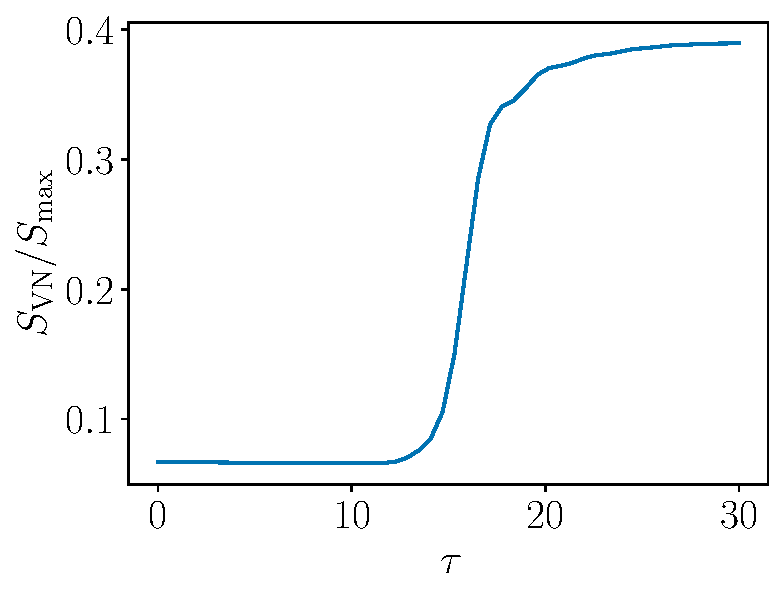
\includegraphics[width=\textwidth]{figures/report_08_2025/entropy_time_exact_Lqpc=60_Omega=0.4_t=0.05.pdf}
        \caption{}
    \end{subfigure}
    \hspace{0.001\textwidth}
    \begin{subfigure}[b]{0.35\textwidth}
        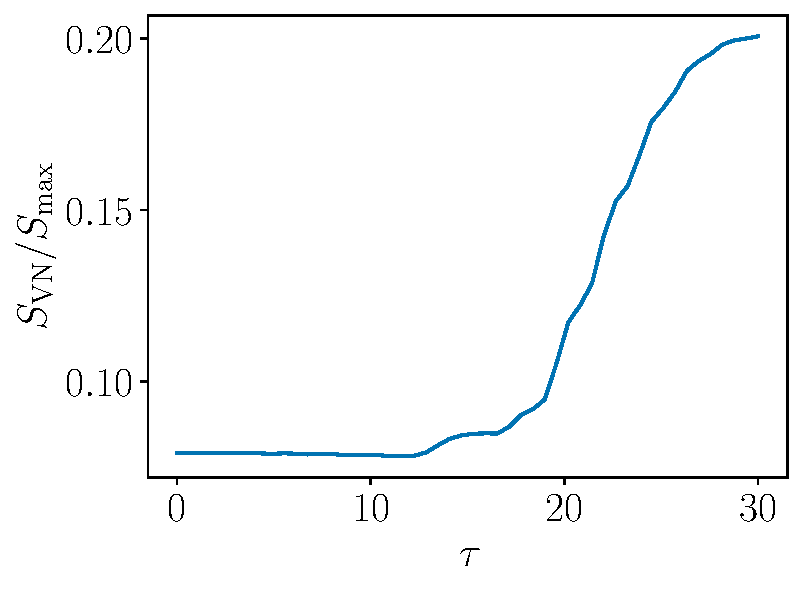
\includegraphics[width=\textwidth]{figures/report_08_2025/entropy_time_exact_Lqpc=60_Omega=0.4_t=0.1.pdf}
        \caption{}
    \end{subfigure}
    \caption{Entanglement entropy a function of time $\tau$ between a QPC Gaussian wave-packet with central momentum $k_0 = \pi/2$ and a qubit. The detector-systems are the same as those shown in figure \ref{fig:energy_bands}, with (a) $t=0.05$ and (b)$t=0.1$. The entropy is normalized by $S_{\rm{max}} = \log(2)$, being the singlet entropy.}
    \label{fig:entropy_in_time}
\end{figure}

Nonetheless, these plots agree with earlier results for smaller $L=21$. The difference is that in the larger system we obtain a better saturation, since we are able to run the simulations for longer time without reflections from the end of the QPC chain.

In figure \ref{fig:wave_packet_entropy} we plot the maximum entropy of the wavepacket as a function of $k_0$, for both $L=60$ and $L=21$ to contrast both cases. While the overall trend of vanishing entropy at $k_0 \approx 0, \pi/2$ is present in both the small and large system, in the latter there is higher entropy and additional effects towards lower momenta. These are likely due to the fact that a longer chain has more available degenerate momenta. To properly account for such finite size effects we have to take the $L\rightarrow \infty$ limit, which goes beyond the applicability of our current perturbative expansion.

\begin{figure}[h]
    \centering
    \begin{subfigure}[b]{0.7\textwidth}
        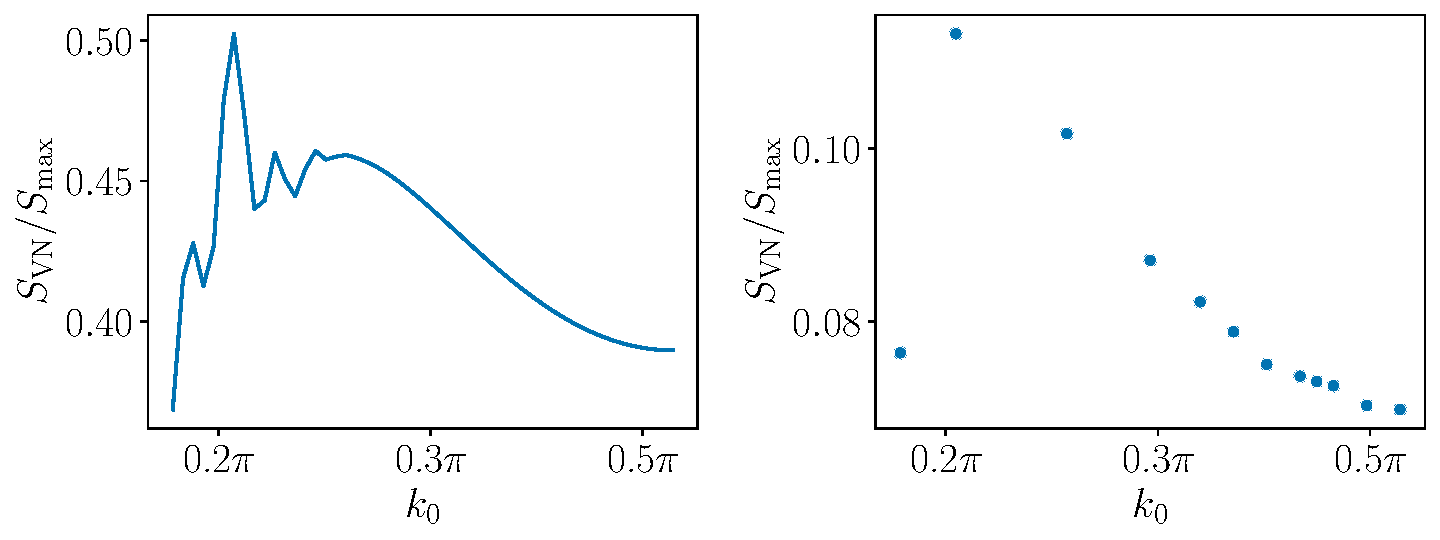
\includegraphics[width=\textwidth]{figures/report_08_2025/wavepacket_entropies_Lqpc=60_Omega=0.4_t=0.05.pdf}
        \caption{}
    \end{subfigure}
    \vspace{0.001\textwidth}
    \begin{subfigure}[b]{0.7\textwidth}
        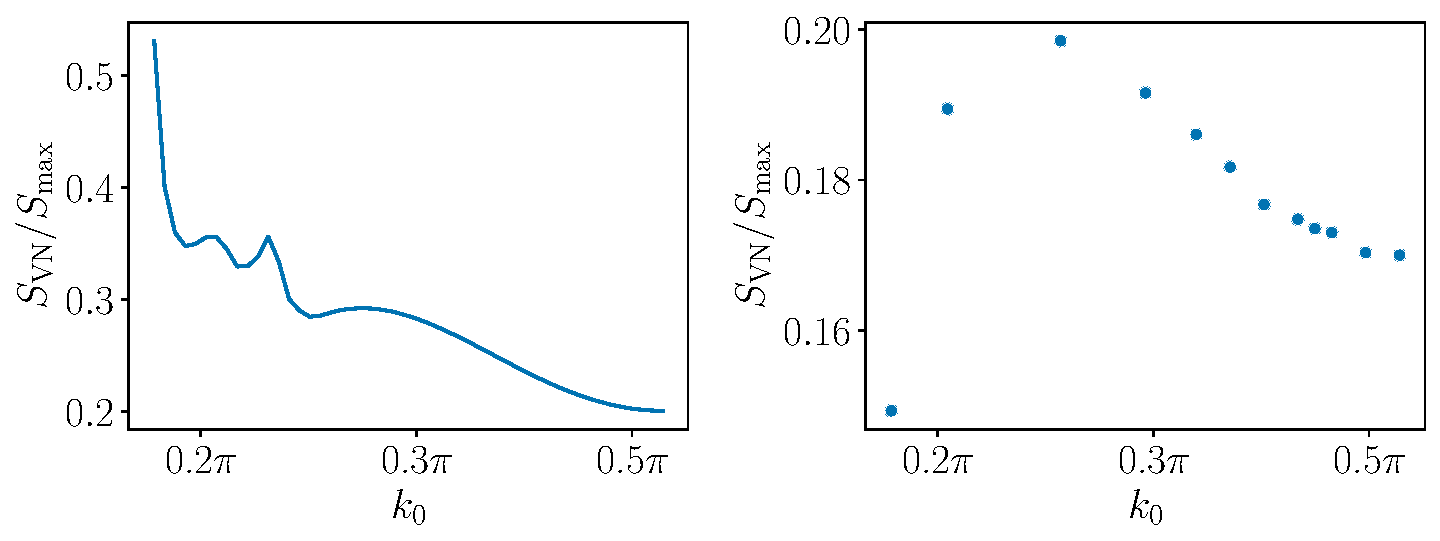
\includegraphics[width=\textwidth]{figures/report_08_2025/wavepacket_entropies_Lqpc=60_Omega=0.4_t=0.1.pdf}
        \caption{}
    \end{subfigure}
    \caption{Maximum Entropy of a wave packet with the same parameters as in figure \ref{fig:entropy_in_time} as a function of $k_0$ for (a) $t=0.05$ and (b) $t=0.1$. The solid lines correspond to a QPC with $L=60$ and the points to $L=21$.}
    \label{fig:wave_packet_entropy}
\end{figure}

As a final note, we can plug the perturbative $\ket{\psi_\nu (k)} = \ket{\psi_\nu^{(0)} (k)} + \Omega \ket{\psi_\nu^{(1)} (k)}$ in Eq.\eqref{eq:mps_wavepacket} to estimate the densities as a function of time. In principle one can also try to compute the entropy, but this just gives nonsense, as a proper estimate involves second order corrections. As a summary, the occupations to the left, right and directly at the bond are shown in figure \ref{fig:occupations} for the two previous cases. In addition, the transmission coefficient
\begin{align}\label{eq:transmission_coef}
T = \left( \frac{\Delta^2}{\pi}\right)^{1/2} \int_{-\infty}^{\infty}  \, dk \frac{e^{-(k-k_{0})^2\Delta^2}}{1+\left(\frac{m V_{0}}{k}\right)^2 },
\end{align}
with $V_0 = J \Omega \langle \hat{n}_0(\tau_{\rm{hit}}) \rangle $, is included. This expression is found by assuming a free Gaussian wavepacket interacting with a $\delta$-potential. Unsurprisingly, the perturbative approximation is much better when $t<0.052$ as it is expected to be well-behaved there. This figure, also shows that the transmission for lower $t$ is much closer to the scattering prediction. Finally, we note that
there are still some leftover oscillations from finite size effects, but in comparison to previous $L=21$ cases these are much more suppressed.

\begin{figure}[h]
    \centering
    \begin{subfigure}[b]{0.7\textwidth}
        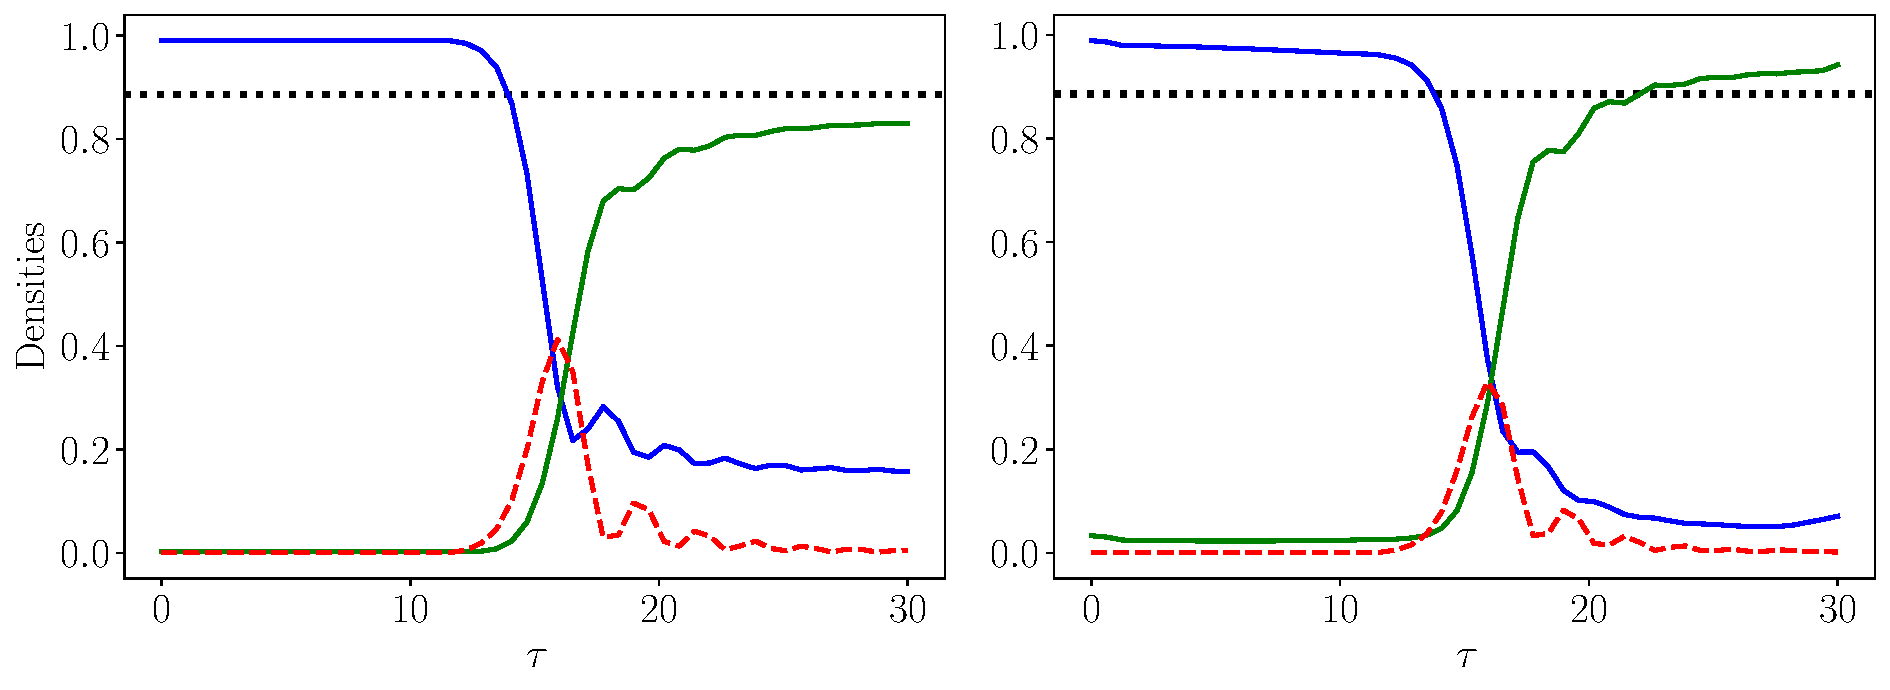
\includegraphics[width=\textwidth]{figures/report_08_2025/occupations_Lqpc=60_Omega=0.4_t=0.05.pdf}
        \caption{}
    \end{subfigure}
    \vspace{0.001\textwidth}
    \begin{subfigure}[b]{0.7\textwidth}
        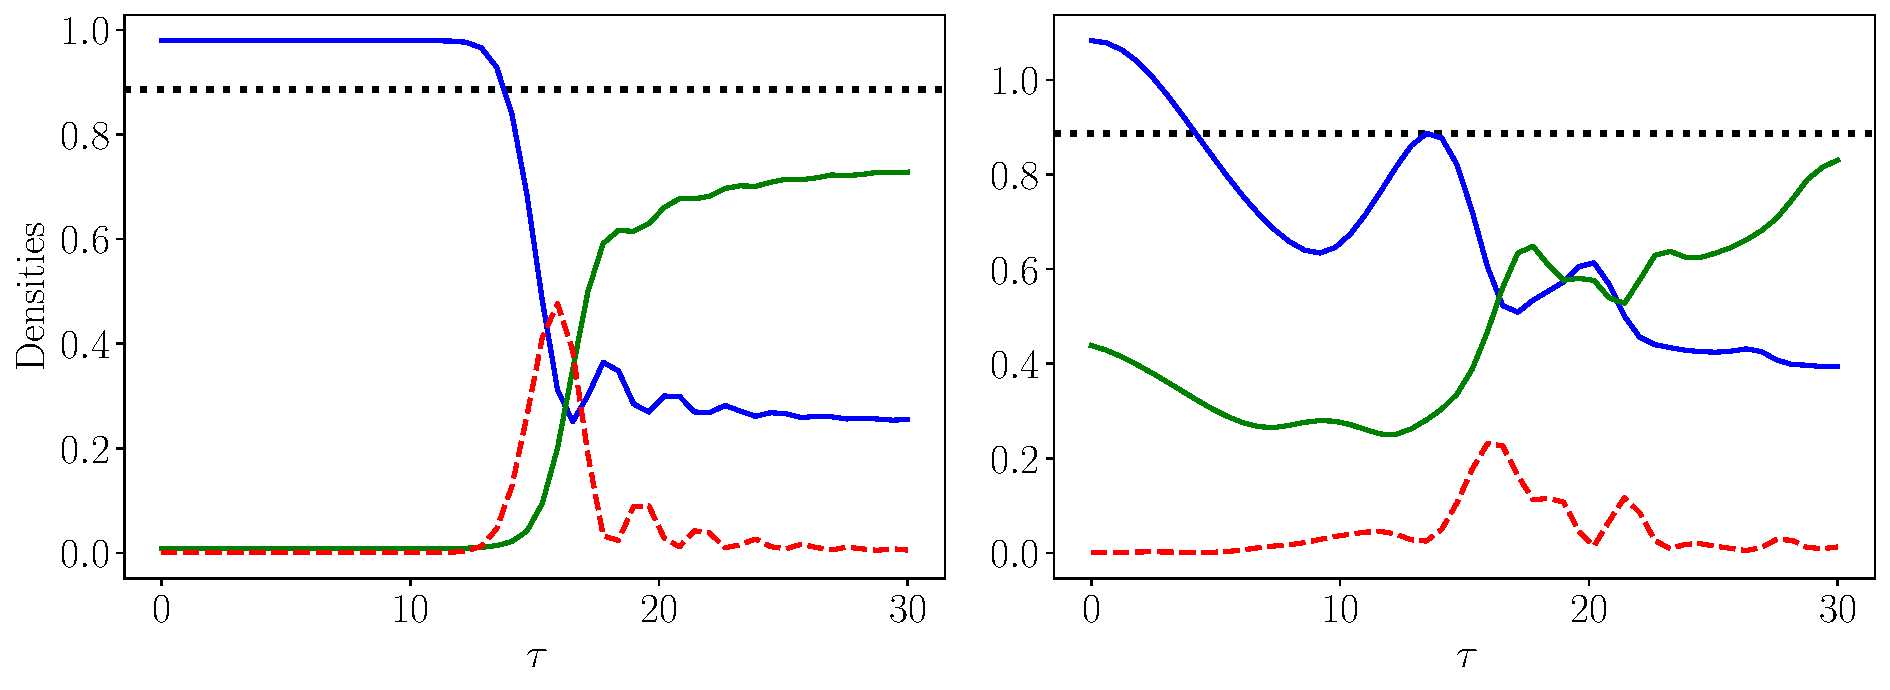
\includegraphics[width=\textwidth]{figures/report_08_2025/occupations_Lqpc=60_Omega=0.4_t=0.1.pdf}
        \caption{}
    \end{subfigure}
    \caption{Occupations for the same system shown in figure \ref{fig:entropy_in_time} where (a) $t=0.05$ and (b) $t=0.1$. The left column depicts the results for the exact eigenstatesm, and the right one the results with the perturbative eigenstates from Eq.\eqref{eq:psi_1}. The blue solid line, represents the occupations to the left of the bond, the green solid line the occupations to the right of the bond and the red dashed lines the occupations directly at the bond. The black dashed lines are the transmission coefficients from Eq.\eqref{eq:transmission_coef}. }
    \label{fig:occupations}
\end{figure}


%\bibliography{qpc}
%\bibliographystyle{ieeetr}


\end{document}